\chapter{Perkembangbiakan Seksual Tumbuhan Berbunga}\label{ch:b2:angiosperm-reproduction}

Sebuah kebun apel pada bulan Mei memutih oleh \omterm{def:b2:angiosperm-reproduction:flower}{bunga} dan riuh oleh
lebah; pada bulan Oktober pohon yang sama sarat oleh \omterm{def:b2:angiosperm-reproduction:seed}{buah}, tiap apelnya
memuat sepuluh \omterm{def:b2:angiosperm-reproduction:seed}{biji}, dan tiap \omterm{def:b2:angiosperm-reproduction:seed}{bijinya} sebatang pohon lembaga yang
terbungkus simpanan makanan. Seluruh perubahan itu --- \omterm{def:b2:angiosperm-reproduction:flower}{bunganya}, \omterm{def:b2:plant-life-cycles:heterospory}{serbuk
sari} yang dibawa serangga, buluh yang tumbuh menembus tangkai putiknya,
\omterm{prop:b2:angiosperm-reproduction:double}{pembuahan ganda} yang sekaligus membuat sebuah lembaga dan pasokan
makanannya, \omterm{def:b2:angiosperm-reproduction:flower}{bakal buah} yang menggembung menjadi \omterm{def:b2:angiosperm-reproduction:seed}{buah} yang dibangun
untuk dimakan --- adalah penemuan yang menjadikan tumbuhan berbunga,
dalam seratus juta tahun, sebagai tumbuhan yang mendominasi daratan.
Bab ini menempuhnya dari \omterm{def:b2:angiosperm-reproduction:flower}{bunga} sampai ke \omterm{def:b2:angiosperm-reproduction:seed}{biji} yang tersebar.

\section{Bunganya}

\begin{definition}[Bagian-bagian sebuah bunga]\label{def:b2:angiosperm-reproduction:flower}
\index{bunga}\index{benang sari}\index{daun buah}\index{bakal buah}\index{kepala putik}
Sebuah \emph{bunga} adalah pucuk pendek yang daunnya berubah menjadi
empat karangan. Di sebelah luar, \emph{daun kelopak} (bersama-sama
kelopaknya) melindungi kuncupnya; lalu \emph{daun mahkota} (mahkotanya),
yang mengiklankan; lalu \emph{benang sari}, masing-masing sebuah tangkai
sari yang mengusung sebuah \emph{kepala sari} berisi empat kantung
\omterm{def:b2:plant-life-cycles:heterospory}{serbuk sari}; dan di pusatnya satu atau beberapa \emph{daun \omterm{def:b2:angiosperm-reproduction:seed}{buah}},
masing-masing terlipat dan tertutup menjadi sebuah \emph{putik} dengan
sebuah \emph{kepala putik} yang siap terima, sebuah \emph{tangkai
putik}, dan sebuah \emph{bakal \omterm{def:b2:angiosperm-reproduction:seed}{buah}} yang mengurung
\emph{\omterm{def:b2:plant-life-cycles:heterospory}{bakal biji}}. Bunga dengan benang sari sekaligus daun \omterm{def:b2:angiosperm-reproduction:seed}{buah}
disebut \emph{hermafrodit} (sebagian besar spesies); tumbuhan
\emph{berumah satu} mengusung bunga jantan dan betina terpisah pada
satu individu (jagung, ek, hazel), sedangkan spesies \emph{berumah dua}
mengusungnya pada individu terpisah (holi, dedalu, kurma). Seluruh
maksud daun \omterm{def:b2:angiosperm-reproduction:seed}{buah} yang tertutup --- ciri yang menamai angiosperma ---
adalah bahwa \omterm{def:b2:plant-life-cycles:heterospory}{bakal bijinya} terkurung: \omterm{def:b2:plant-life-cycles:heterospory}{serbuk sarinya} tidak pernah
mencapainya langsung, melainkan harus tumbuh menuju kepadanya menembus
jaringan tumbuhannya, dan itu membiarkan tumbuhannya memilih.
\end{definition}

\begin{omfigure}
\begin{tikzpicture}[every node/.style={font=\scriptsize}]
  % receptacle and pedicel
  \draw[thick] (0,-2.6) -- (0,-1.6);
  \draw[thick, fill=omExo!20] (-0.9,-1.6) .. controls (-1.0,-1.0) and (1.0,-1.0) .. (0.9,-1.6) -- cycle;
  % sepals
  \foreach \s in {-1,1} \draw[thick, fill=omExo!45] (0.6*\s,-1.4) .. controls (2.0*\s,-1.2) and (2.6*\s,-0.2) .. (2.8*\s,0.6) .. controls (2.0*\s,0.2) and (1.2*\s,-0.6) .. (0.6*\s,-1.4);
  % petals
  \foreach \s in {-1,1} \draw[thick, fill=omThm!15] (0.5*\s,-1.2) .. controls (1.6*\s,0.4) and (2.2*\s,1.8) .. (1.6*\s,3.0) .. controls (1.0*\s,2.0) and (0.5*\s,0.8) .. (0.5*\s,-1.2);
  % ovary with ovules
  \draw[thick, fill=omDef!12] (0,-0.7) ellipse (0.55 and 0.75);
  \foreach \p in {(-0.22,-0.5),(-0.22,-0.9),(0.22,-0.5),(0.22,-0.9)} \draw[thick, omDef, fill=omDef!40] \p circle (0.11);
  % style and stigma
  \draw[thick, fill=omDef!12] (-0.1,0.05) rectangle (0.1,1.9);
  \draw[thick, fill=omDef!40] (0,2.0) ellipse (0.28 and 0.14);
  % stamens
  \foreach \s in {-1,1} { \draw[thick] (0.35*\s,-1.0) .. controls (0.6*\s,0.2) .. (0.9*\s,1.5); \draw[thick, fill=omProp!60] (0.9*\s,1.6) ellipse (0.14 and 0.32); }
  % labels: right side
  \draw (0.28,2.0) -- (3.2,2.6) node[right] {kepala putik};
  \draw (0.1,1.2) -- (3.2,1.9) node[right] {tangkai putik};
  \draw (0.55,-0.6) -- (3.2,1.2) node[right] {bakal buah};
  \draw (0.22,-0.9) -- (3.2,0.5) node[right] {bakal biji};
  \draw (2.6,0.35) -- (3.2,-0.4) node[right] {daun kelopak};
  % labels: left side
  \draw (-1.5,2.4) -- (-2.6,2.8) node[left] {daun mahkota};
  \draw (-0.95,1.9) -- (-2.6,1.9) node[left] {kepala sari};
  \draw (-0.65,0.6) -- (-2.6,0.9) node[left] {tangkai sari};
  \draw (0,-2.2) -- (-2.6,-2.2) node[left] {dasar dan tangkainya};
  \node[anchor=west, align=left] at (5.4,0.5) {kepala putik + tangkai + bakal buah\\$=$ daun buah};
  \node[anchor=west, align=left] at (5.4,-0.8) {kepala sari + tangkai sari\\$=$ benang sarinya};
\end{tikzpicture}

{\small Sebuah \omterm{def:b2:angiosperm-reproduction:flower}{bunga} dalam potongan membujur: daun kelopak, daun
mahkota, \omterm{def:b2:angiosperm-reproduction:flower}{benang sari} (tangkai sari dan kepala sari) dan, di pusatnya,
\omterm{def:b2:angiosperm-reproduction:flower}{daun buahnya} --- \omterm{def:b2:angiosperm-reproduction:flower}{kepala putik}, tangkai putik, dan \omterm{def:b2:angiosperm-reproduction:flower}{bakal buah} --- yang
mengurung \omterm{def:b2:plant-life-cycles:heterospory}{bakal bijinya}.}
\end{omfigure}

\begin{omfigure}
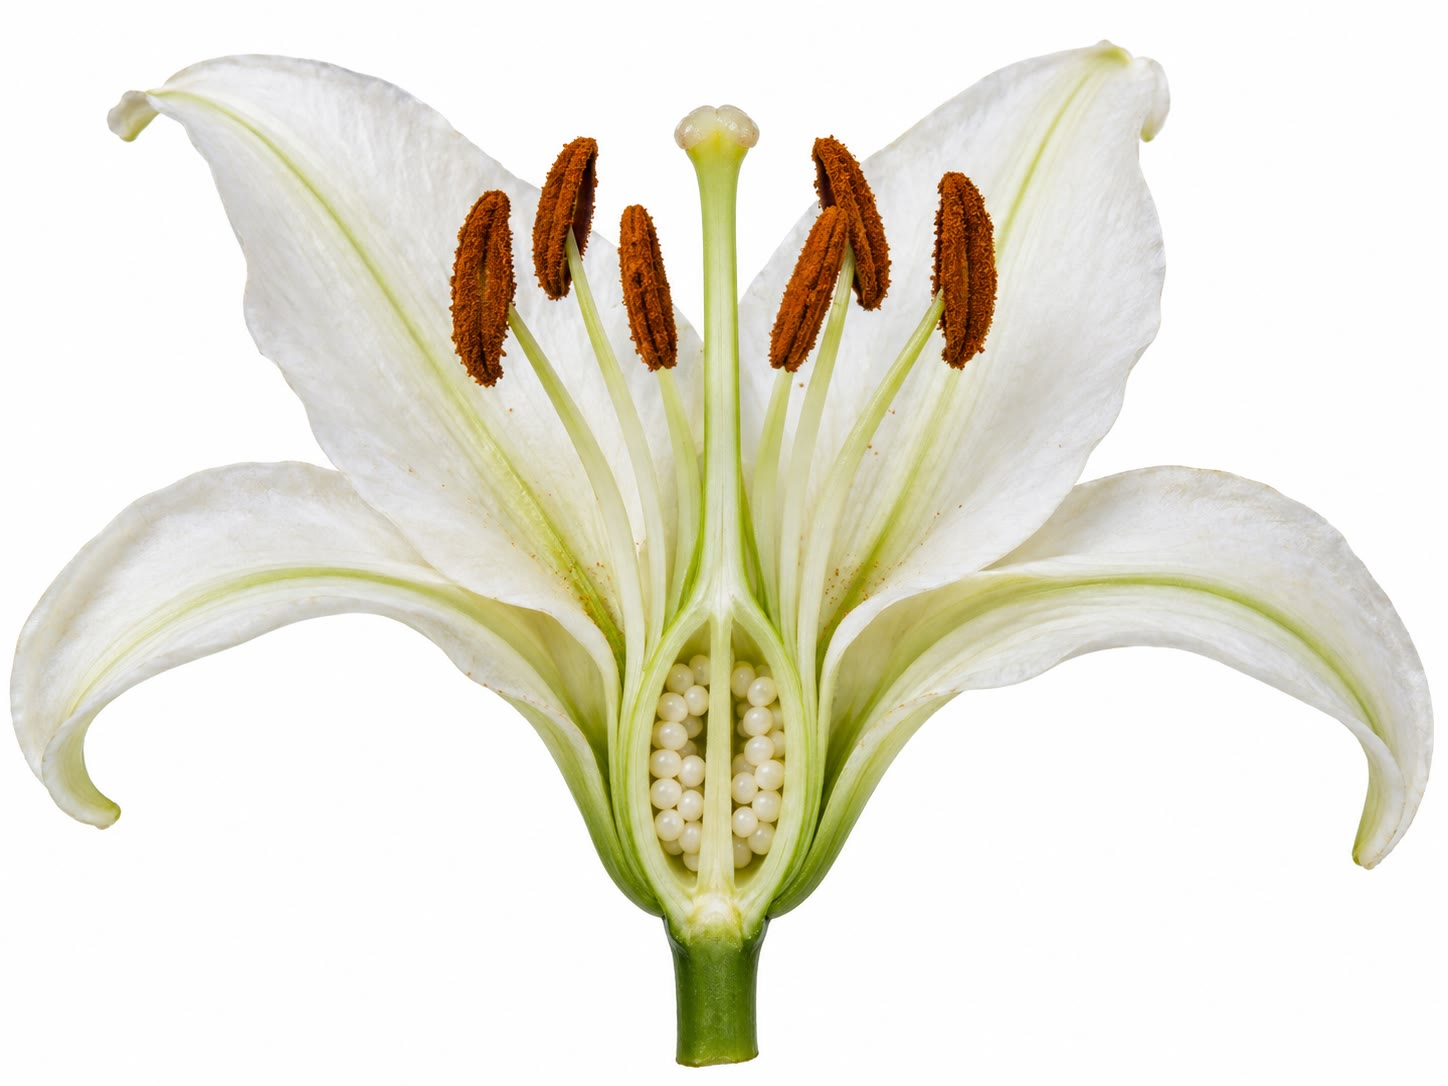
\includegraphics[width=0.55\linewidth]{images/book4/ai/b4-06-lily-dissected.jpg}

{\small Sekuntum bakung dibelah membujur: enam \omterm{def:b2:angiosperm-reproduction:flower}{benang sari} dengan
kepala sari yang sarat \omterm{def:b2:plant-life-cycles:heterospory}{serbuk sari}, tangkai putiknya yang panjang
dengan \omterm{def:b2:angiosperm-reproduction:flower}{kepala putiknya} yang lengket, dan \omterm{def:b2:angiosperm-reproduction:flower}{bakal buahnya} yang dibuka
untuk memperlihatkan deretan \omterm{def:b2:plant-life-cycles:heterospory}{bakal bijinya}.}
\end{omfigure}

\section{Kedua gametofitnya}

\begin{proposition}[Serbuk sari: gametofit jantannya]\label{prop:b2:angiosperm-reproduction:pollen}
\index{butir serbuk sari}\index{mikrosporogenesis}\index{sporopolenin}
Di dalam tiap kantung \omterm{def:b2:plant-life-cycles:heterospory}{serbuk sari}, sel induk yang \omterm{def:b2:meiosis-heredity:meiosis}{diploid} menjalani
\omterm{def:b2:meiosis-heredity:meiosis}{meiosis} sehingga memberi tetrad \emph{\omterm{def:b2:plant-life-cycles:heterospory}{mikrospora}}. Tiap \omterm{def:b2:plant-life-cycles:heterospory}{mikrospora}
membelah sekali, secara tak setara, menjadi sebuah \emph{sel
vegetatif} yang besar dan sebuah \emph{sel generatif} yang kecil yang
terkurung di dalamnya; sel generatifnya membelah sekali lagi, sebelum
atau sesudah \omterm{def:b2:angiosperm-reproduction:pollination}{penyerbukan}, menjadi dua \emph{sel sperma}.
\emph{\omterm{prop:b2:angiosperm-reproduction:pollen}{Butir serbuk sari}} yang matang dengan demikian adalah organisme
\omterm{def:b2:meiosis-heredity:meiosis}{haploid} bersel tiga --- seluruh \omterm{def:b2:plant-life-cycles:cycles}{gametofit} jantannya --- berukuran
\qtyrange{10}{100}{\micro m}, tertutup sebuah dinding yang lapisan
luarnya, \emph{sporopolenin}, polimer biologis paling tahan yang
dikenal, dipahat dengan duri, liang, dan alur yang khas bagi
spesiesnya, dan itulah sebabnya \omterm{def:b2:plant-life-cycles:heterospory}{serbuk sari} mengenali tumbuhan di dalam
endapan berumur puluhan juta tahun. Butirnya dilepaskan dalam keadaan
tanpa air, dan bertahan berjam-jam (rumput) sampai berpekan-pekan
(sebagian pohon) sampai ia mencapai sebuah \omterm{def:b2:angiosperm-reproduction:flower}{kepala putik}.
\end{proposition}

\begin{omfigure}
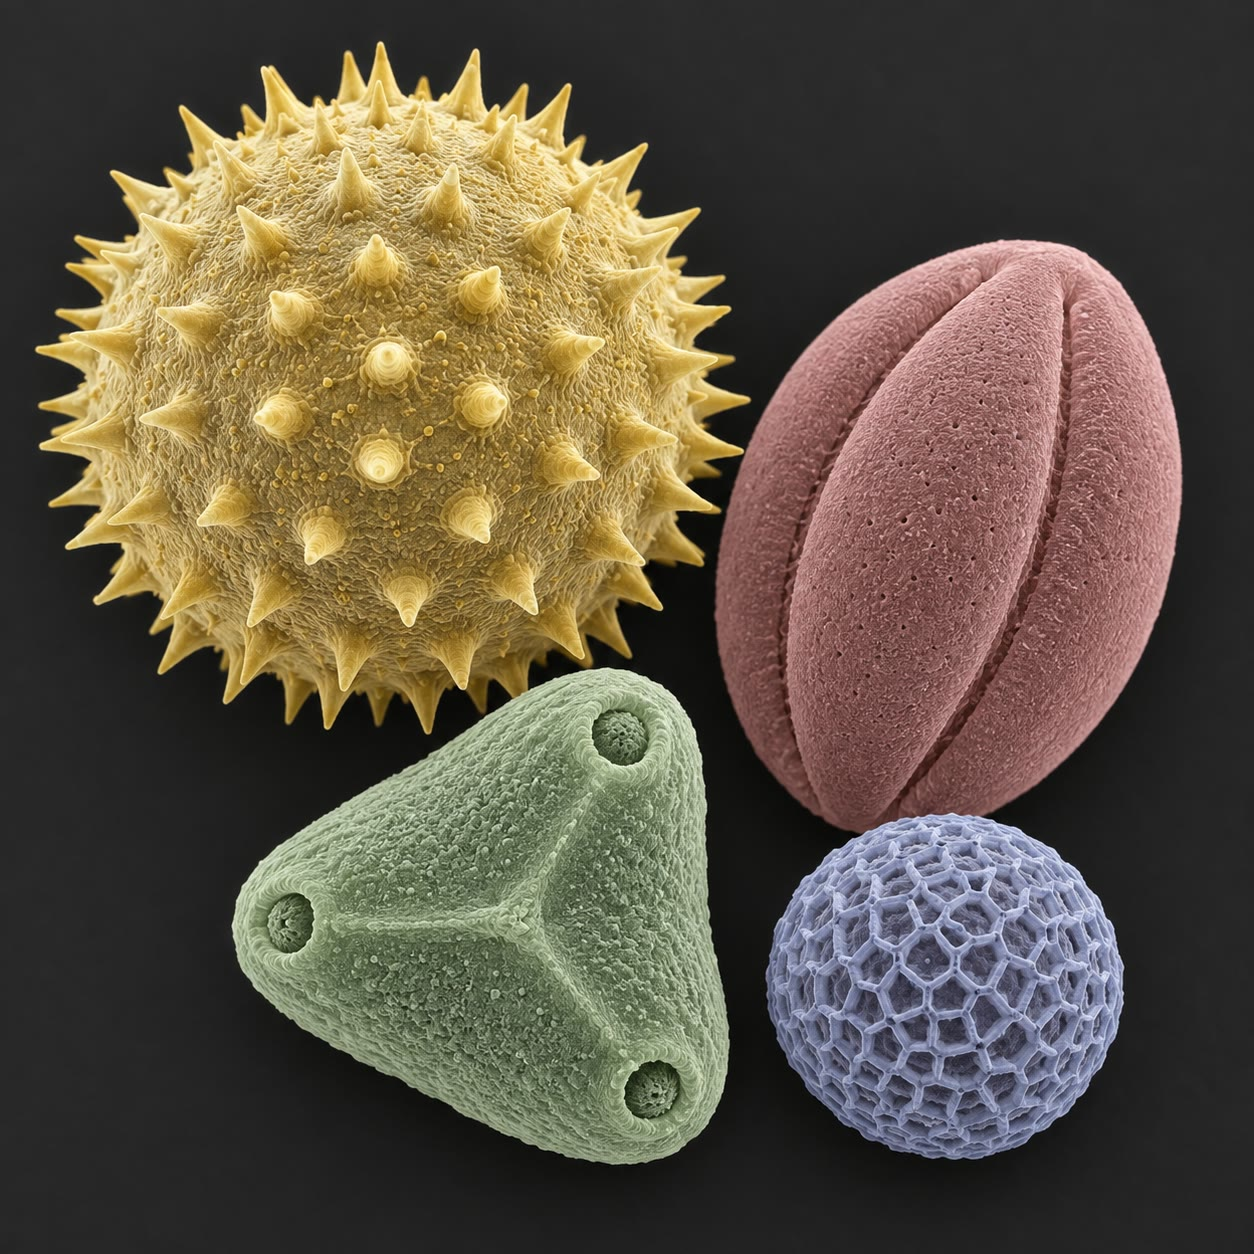
\includegraphics[width=0.45\linewidth]{images/book4/ai/b4-06-pollen-sem.jpg}

{\small \omterm{prop:b2:angiosperm-reproduction:pollen}{Butir serbuk sari} di bawah mikroskop elektron payaran: dinding
sporopolenin tiap spesiesnya memiliki pahatannya sendiri --- duri,
alur, liang, jala --- dan darinya ia dapat dikenali.}
\end{omfigure}

\begin{proposition}[Kantung lembaga: gametofit betinanya]\label{prop:b2:angiosperm-reproduction:embryosac}
\index{kantung lembaga}\index{megasporogenesis}\index{inti kutub}
Di dalam tiap \omterm{def:b2:plant-life-cycles:heterospory}{bakal biji}, satu sel \omterm{def:b2:meiosis-heredity:meiosis}{diploid} nuselusnya menjalani
\omterm{def:b2:meiosis-heredity:meiosis}{meiosis}; tiga dari keempat \omterm{def:b2:plant-life-cycles:heterospory}{megasporanya} merosot dan yang keempat
tumbuh, lewat tiga mitosis tanpa pembelahan sel, menjadi sebuah
\emph{\omterm{prop:b2:angiosperm-reproduction:embryosac}{kantung lembaga}} berinti delapan dan bersel tujuh: pada ujung
mikropilnya terdapat \emph{sel telur} yang diapit dua
\emph{sinergid}; pada ujung seberangnya tiga sel \emph{antipoda}; dan
di tengahnya sebuah \emph{sel pusat} besar yang memuat dua
\emph{\omterm{prop:b2:angiosperm-reproduction:embryosac}{inti kutub}}. Kantung ini, yang terbungkus nuselus dan dua
integumen bermikropil, adalah seluruh \omterm{def:b2:plant-life-cycles:cycles}{gametofit} betinanya --- tujuh sel
di tempat \omterm{def:b2:plant-life-cycles:moss}{lumut} memiliki satu tumbuhan. Kedua \omterm{prop:b2:angiosperm-reproduction:embryosac}{inti kutubnya} serupa
secara genetik dengan sel telurnya, dan kenyataan itu berarti bagi
endospermanya.
\end{proposition}

\begin{omfigure}
\begin{tikzpicture}[every node/.style={font=\scriptsize}]
  % pollen grain
  \begin{scope}
    \draw[very thick, omProp!80!black, fill=omProp!15] (0,0) circle (1.1);
    \draw[thick, omProp!80!black] (0,0) circle (0.95);
    \foreach \a in {0,30,...,330} \draw[omProp!80!black, thick] (\a:1.1) -- (\a:1.25);
    \draw[thick, fill=omDef!25] (0.15,-0.2) ellipse (0.55 and 0.4); \node[font=\tiny] at (0.15,-0.2) {vegetatif};
    \draw[thick, fill=omThm!30] (-0.3,0.45) ellipse (0.22 and 0.14); \draw[thick, fill=omThm!30] (0.2,0.5) ellipse (0.22 and 0.14);
    \draw[omThm] (0.0,0.62) -- (0.0,1.5); \node[omThm, anchor=south] at (0.0,1.5) {dua sel sperma};
    \node[below, align=center] at (0,-1.4) {butir serbuk sari ($n$)\\3 sel, dinding sporopolenin};
  \end{scope}
  % ovule with embryo sac
  \begin{scope}[xshift=5.5cm]
    \draw[thick, fill=omExo!25] (0,0) ellipse (1.5 and 2.1);
    \draw[thick, fill=omExo!10] (0,0) ellipse (1.15 and 1.75);
    \fill[white] (-0.3,1.7) rectangle (0.3,2.2); \draw[thick] (-0.3,1.7) -- (-0.3,2.15); \draw[thick] (0.3,1.7) -- (0.3,2.15);
    \draw[thick, fill=white] (0,0) ellipse (0.7 and 1.35);
    % cells: egg + synergids top, central, antipodals bottom
    \draw[thick, fill=omThm!30] (0,0.95) circle (0.17); \node[omThm, anchor=west] at (1.6,1.2) {sel telur};
    \draw[thick, fill=omDef!25] (-0.35,1.0) circle (0.14); \draw[thick, fill=omDef!25] (0.35,1.0) circle (0.14); \node[anchor=west] at (1.6,0.75) {dua sinergid};
    \draw[thick, fill=omDef!10] (0,0) ellipse (0.55 and 0.6); \fill[omDef!80!black] (-0.15,0.05) circle (0.09); \fill[omDef!80!black] (0.15,0.05) circle (0.09);
    \node[anchor=west, align=left] at (1.6,0.1) {sel pusat dengan\\dua inti kutub};
    \foreach \x in {-0.3,0,0.3} \draw[thick, fill=omDef!25] (\x,-1.0) circle (0.13); \node[anchor=west] at (1.6,-1.0) {tiga antipoda};
    \draw (0.35,2.0) -- (1.6,2.0) node[right] {mikropil};
    \draw (1.3,-0.9) -- (1.6,-1.6) node[right] {integumen};
    \draw (0.9,-1.35) -- (1.6,-2.1) node[right] {nuselus};
    \draw (1.6,1.2) -- (0.17,0.95); \draw (1.6,0.75) -- (0.49,1.0); \draw (1.6,0.1) -- (0.55,0.05); \draw (1.6,-1.0) -- (0.43,-1.0);
    \node[below, align=center] at (0,-2.3) {bakal biji dengan kantung lembaga ($n$)\\7 sel, 8 inti};
  \end{scope}
\end{tikzpicture}

{\small Kedua \omterm{def:b2:plant-life-cycles:cycles}{gametofit} sebatang tumbuhan berbunga, keduanya menyusut
menjadi beberapa sel: \omterm{prop:b2:angiosperm-reproduction:pollen}{butir serbuk sari} bersel tiga, dan \omterm{prop:b2:angiosperm-reproduction:embryosac}{kantung
lembaga} bersel tujuh di dalam \omterm{def:b2:plant-life-cycles:heterospory}{bakal bijinya}.}
\end{omfigure}

\section{Penyerbukan}

\begin{definition}[Penyerbukan dan pelakunya]\label{def:b2:angiosperm-reproduction:pollination}
\index{penyerbukan}\index{sindrom penyerbukan}\index{nektar}
\emph{Penyerbukan} adalah pemindahan \omterm{def:b2:plant-life-cycles:heterospory}{serbuk sari} dari sebuah kepala
sari ke sebuah \omterm{def:b2:angiosperm-reproduction:flower}{kepala putik}; \emph{penyerbukan sendiri} terjadi di
dalam satu \omterm{def:b2:angiosperm-reproduction:flower}{bunga} atau satu tumbuhan, \emph{penyerbukan silang} antar
tumbuhan. \omterm{def:b2:angiosperm-reproduction:flower}{Bunga} yang \emph{diserbuki angin} (rumput, ek, birka,
sendokan) berukuran kecil, hijau, tak berbau, dengan \omterm{def:b2:angiosperm-reproduction:flower}{kepala putik}
berbulu yang besar dan \omterm{def:b2:plant-life-cycles:heterospory}{serbuk sari} kering serta licin dalam jumlah luar
biasa banyak; rasio \omterm{def:b2:plant-life-cycles:heterospory}{serbuk sari} terhadap \omterm{def:b2:plant-life-cycles:heterospory}{bakal bijinya} mencapai
sejuta. \omterm{def:b2:angiosperm-reproduction:flower}{Bunga} yang \emph{diserbuki hewan} membayar pengangkutnya:
\emph{nektar} (larutan gula dari kelenjar madu), \omterm{def:b2:plant-life-cycles:heterospory}{serbuk sari} itu
sendiri, minyak, dan wangi; dan mereka mengiklankan diri dengan warna,
bentuk, serta bau yang ditala kepada indra pengangkutnya --- penuntun
nektar ultraungu bagi lebah, yang melihat ultraungu dan tidak melihat
merah; \omterm{def:b2:angiosperm-reproduction:flower}{bunga} tabung merah tanpa wangi bagi burung kolibri; \omterm{def:b2:angiosperm-reproduction:flower}{bunga}
putih, sangat wangi, yang mekar malam hari dengan tabung yang dalam
bagi ngengat; \omterm{def:b2:angiosperm-reproduction:flower}{bunga} cokelat berbau busuk bagi lalat bangkai; \omterm{def:b2:angiosperm-reproduction:flower}{bunga}
malam yang kukuh dan pucat bagi kelelawar. Tiap perangkat ciri semacam
itu adalah sebuah \emph{sindrom penyerbukan}, dan kecocokan antara
\omterm{def:b2:angiosperm-reproduction:flower}{bunga} dan penyerbuknya adalah contoh buku teks \emph{koevolusi}: dari
taji nektar \qty{30}{cm} sebuah anggrek Madagaskar, Darwin meramalkan
seekor ngengat berlidah \qty{30}{cm}, yang ditemukan empat puluh tahun
kemudian.
\end{definition}

\begin{omfigure}
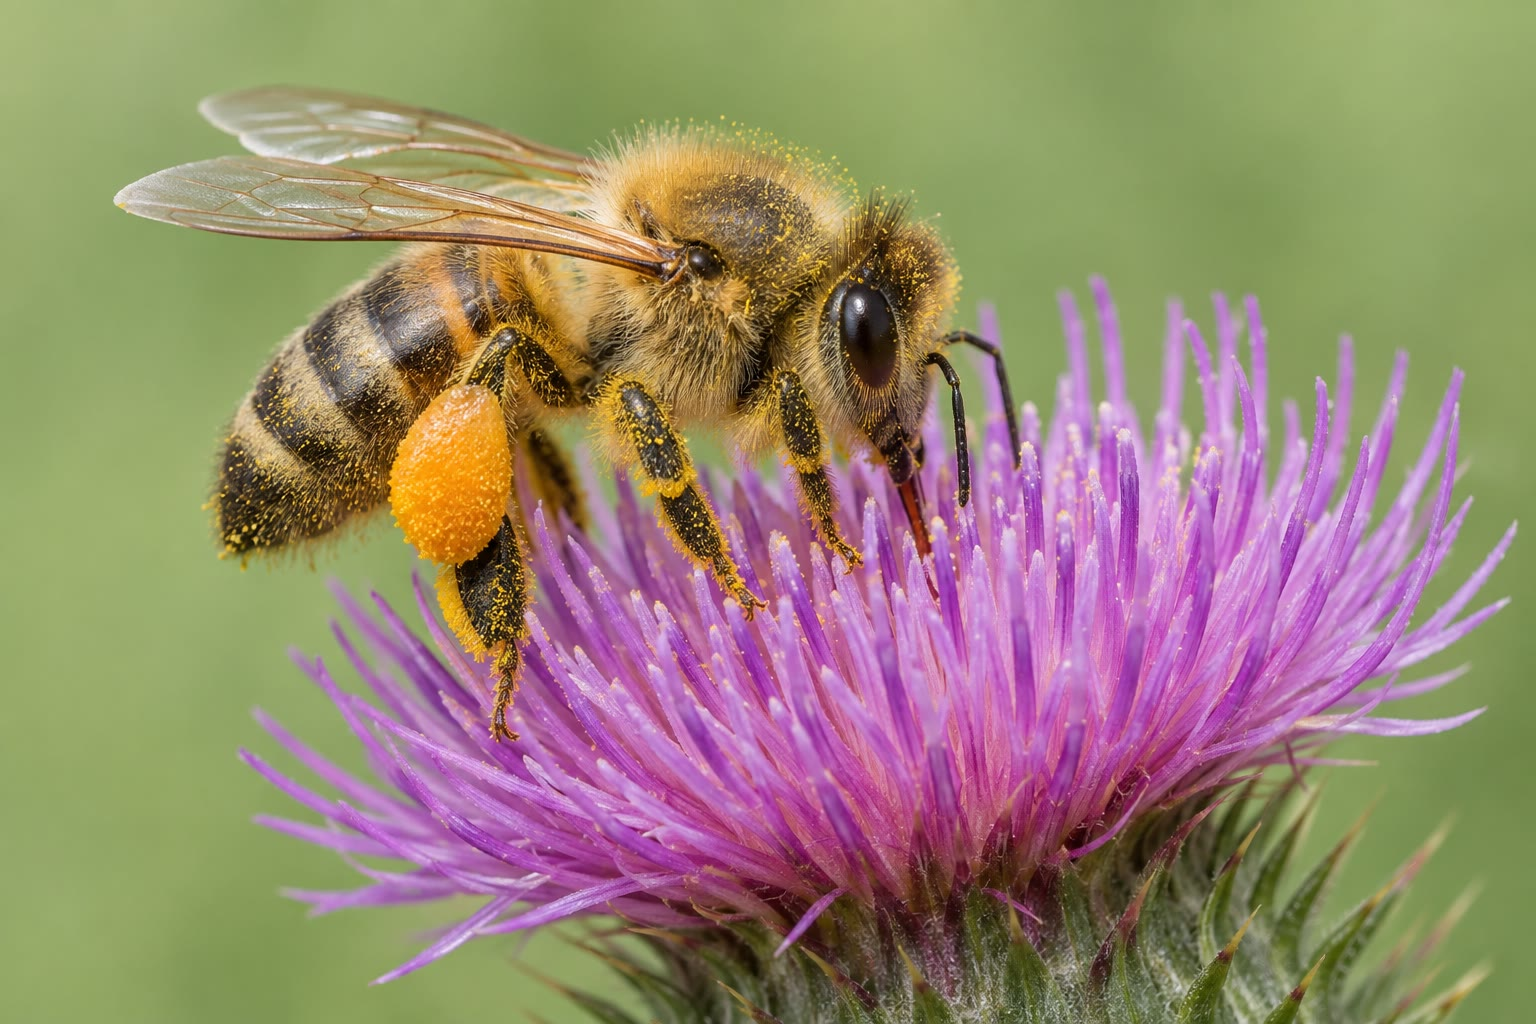
\includegraphics[width=0.58\linewidth]{images/book4/ai/b4-06-bee-on-flower.jpg}

{\small Seekor lebah madu pada sekuntum \omterm{def:b2:angiosperm-reproduction:flower}{bunga} rumput teki: \omterm{def:b2:plant-life-cycles:heterospory}{serbuk sari}
menaburi tubuhnya dan memenuhi keranjang kaki belakangnya; sebagian
darinya akan mencapai \omterm{def:b2:angiosperm-reproduction:flower}{kepala putik} \omterm{def:b2:angiosperm-reproduction:flower}{bunga} berikutnya yang
dikunjunginya. Warna ungu, landasan pendaratan, dan \omterm{def:b2:angiosperm-reproduction:pollination}{nektar} yang
berlimpah adalah sindrom lebah.}
\end{omfigure}

\begin{proposition}[Menghindari pembuahan sendiri]\label{prop:b2:angiosperm-reproduction:selfing}
\index{ketakserasian sendiri}\index{heterostili}\index{dikogami}
Sebuah \omterm{def:b2:angiosperm-reproduction:flower}{bunga} hermafrodit dapat membuahi dirinya sendiri, dan banyak
yang melakukannya (kacang ercis, gandum, tomat); tetapi pembuahan
sendiri menyingkapkan \omterm{def:b2:meiosis-heredity:vocabulary}{alel} \omterm{def:b2:meiosis-heredity:vocabulary}{resesif} yang merugikan (\emph{depresi
silang dalam}), dan sebagian besar spesies mencegahnya. Dalam waktu:
\emph{dikogami}, yaitu kepala sari dan \omterm{def:b2:angiosperm-reproduction:flower}{kepala putik} yang matang pada
waktu yang berbeda (protandri pada sebagian besar suku adas dan suku
kenikir). Dalam ruang: \emph{herkogami}, yaitu kepala sari dan \omterm{def:b2:angiosperm-reproduction:flower}{kepala
putik} yang ditempatkan berjauhan, seperti pada \emph{heterostili}
\omterm{def:b2:angiosperm-reproduction:flower}{bunga} primula, yang \omterm{def:b2:angiosperm-reproduction:flower}{bunga} pinnya (tangkai putik panjang, kepala sari
rendah) dan \omterm{def:b2:angiosperm-reproduction:flower}{bunga} trumnya (tangkai putik pendek, kepala sari tinggi)
menaruh \omterm{def:b2:plant-life-cycles:heterospory}{serbuk sari} pada bagian serangga yang berbeda. Secara
biokimia: \emph{\omterm{prop:b2:angiosperm-reproduction:selfing}{ketakserasian sendiri}}, yaitu sistem pengenalan yang di
dalamnya \omterm{def:b2:plant-life-cycles:heterospory}{serbuk sari} yang mengusung \omterm{def:b2:meiosis-heredity:vocabulary}{alel} $S$ yang sama dengan putiknya
ditolak. Pada ketakserasian \emph{gametofitik} (apel, ceri, petunia,
rumput), \omterm{def:b2:meiosis-heredity:vocabulary}{alel} $S$ \omterm{def:b2:meiosis-heredity:meiosis}{haploid} \omterm{def:b2:plant-life-cycles:heterospory}{serbuk sarinya} sendiri yang memutuskan:
putik $S_1S_2$ menghentikan buluh $S_1$ dan $S_2$ di dalam tangkai
putiknya, sehingga \omterm{def:b2:plant-life-cycles:heterospory}{serbuk sari} dari tumbuhan $S_1S_3$ separuhnya serasi
dan dari $S_3S_4$ seluruhnya serasi. Pada ketakserasian
\emph{sporofitik} (kubis, bunga matahari), \omterm{def:b2:meiosis-heredity:vocabulary}{genotipe} \omterm{def:b2:meiosis-heredity:meiosis}{diploid} tetua
\omterm{def:b2:plant-life-cycles:heterospory}{serbuk sarinya} yang memutuskan, pada permukaan \omterm{def:b2:angiosperm-reproduction:flower}{kepala putiknya}. Sebuah
\omterm{def:b2:meiosis-heredity:vocabulary}{alel} $S$ yang langka serasi dengan hampir setiap pasangan, sehingga
seleksi mempertahankan puluhan \omterm{def:b2:meiosis-heredity:vocabulary}{alel} di dalam sebuah populasi.
\end{proposition}
\begin{proof}[Bukti eksperimental]
Darwin (1862, 1877) menyilangkan \omterm{def:b2:angiosperm-reproduction:flower}{bunga} primula dengan tangan: \omterm{def:b2:plant-life-cycles:heterospory}{serbuk
sari} dari \omterm{def:b2:angiosperm-reproduction:flower}{bunga} trum pada \omterm{def:b2:angiosperm-reproduction:flower}{kepala putik} pin (perpaduan yang ``sah'')
menghasilkan kapsul yang penuh; pin pada pin atau trum pada trum
(``tak sah'') menghasilkan sedikit \omterm{def:b2:angiosperm-reproduction:seed}{biji} atau sama sekali tidak,
meskipun tumbuhannya sehat dan \omterm{def:b2:plant-life-cycles:heterospory}{serbuk sarinya} hidup. Ia menyimpulkan
bahwa kedua bentuknya saling teradaptasi untuk menyilang dan terlindung
dari pembuahan sendiri, dan dengan mencacah \omterm{def:b2:angiosperm-reproduction:seed}{biji} tiap kapsul pada
ribuan persilangan ia mengukur ongkos pembuahan sendiri pada puluhan
spesies: keturunan hasil pembuahan sendiri lebih pendek, lebih ringan,
dan kurang subur, generasi demi generasi.
\end{proof}

\begin{omfigure}
\begin{tikzpicture}[every node/.style={font=\scriptsize}]
  % pistil S1S2 with pollen tubes
  \draw[thick, fill=omDef!10] (-0.5,0) rectangle (0.5,3.2);
  \draw[thick, fill=omDef!30] (0,3.3) ellipse (0.7 and 0.2);
  \draw[thick, fill=omDef!12] (0,-0.6) ellipse (0.9 and 0.7);
  \node at (0,-0.6) {bakal buah};
  \node[anchor=east] at (-1.1,3.3) {kepala putik tumbuhan $S_1S_2$};
  % pollen grains
  \draw[thick, fill=omThm!40] (-0.35,3.75) circle (0.13); \node[omThm, left] at (-0.5,3.75) {$S_1$};
  \draw[thick, fill=omThm!40] (0,3.75) circle (0.13); \node[omThm, anchor=south] at (0,3.92) {$S_2$};
  \draw[thick, fill=omExo!70!black] (0.35,3.75) circle (0.13); \node[right] at (0.5,3.75) {$S_3$};
  % tubes: S1 and S2 stop in the style, S3 reaches the ovary
  \draw[thick, omThm] (-0.35,3.3) -- (-0.35,2.3); \node[omThm, left, align=right] at (-0.55,2.3) {buluh $S_1$\\terhenti};
  \draw[thick, omThm] (0,3.3) -- (0,2.0);
  \draw[thick, omExo!70!black] (0.35,3.3) -- (0.35,-0.2) -- (0.2,-0.5);
  \node[right, align=left] at (0.55,0.9) {buluh $S_3$\\mencapai bakal biji};
  \node[anchor=west, align=left, text width=6cm] at (3.2,3.2) {ketakserasian sendiri gametofitik: buluh serbuk sari yang alel $S$-nya sendiri cocok dengan salah satu alel putiknya dihentikan di dalam tangkai putiknya};
  \node[anchor=west, align=left, text width=6cm] at (3.2,1.4) {serbuk sari dari tumbuhan $S_1S_2$: 0 yang serasi\\dari $S_1S_3$: separuhnya\\dari $S_3S_4$: semuanya};
\end{tikzpicture}

{\small \omterm{prop:b2:angiosperm-reproduction:selfing}{Ketakserasian sendiri} gametofitik. Pada putik $S_1S_2$, buluh
yang mengusung $S_1$ atau $S_2$ terhenti di dalam tangkai putiknya;
sebuah buluh $S_3$ tumbuh sampai ke \omterm{def:b2:angiosperm-reproduction:flower}{bakal buahnya}.}
\end{omfigure}

\section{Pembuahan}

\begin{theorem}[Buluh serbuk sari]\label{thm:b2:angiosperm-reproduction:tube}
\index{buluh serbuk sari}
Sebutir \omterm{def:b2:plant-life-cycles:heterospory}{serbuk sari} pada \omterm{def:b2:angiosperm-reproduction:flower}{kepala putik} yang serasi menyerap air kembali
lalu menumbuhkan sebuah \emph{\omterm{thm:b2:angiosperm-reproduction:tube}{buluh serbuk sari}}: sel vegetatifnya
memanjang lewat pertumbuhan ujung, meletakkan dinding baru pada
puncaknya dengan laju \qtyrange{0.1}{1}{cm/h}, mencerna jalannya
menembus jaringan penghantar tangkai putiknya sambil memakannya.
Buluhnya mengusung kedua sel spermanya pada ujungnya; ia dituntun pada
jarak terakhirnya oleh peptida yang disekresikan sinergidnya, memasuki
\omterm{def:b2:plant-life-cycles:heterospory}{bakal bijinya} lewat mikropilnya, pecah ke dalam salah satu sinergidnya,
lalu melepaskan spermanya. Sebuah buluh yang melintasi tangkai putik
sepanjang $L$ pada kelajuan $v$ memakan $L/v$: beberapa jam pada
sebatang ceri, sehari penuh pada jagung, yang ``rambutnya'' adalah
tangkai putik sepanjang \qty{20}{cm}. Daya hidup \omterm{def:b2:plant-life-cycles:heterospory}{serbuk sari} menetapkan
sebuah jam: \omterm{def:b2:plant-life-cycles:heterospory}{serbuk sari} rumput mati dalam hitungan jam, sehingga
sebuah \omterm{def:b2:angiosperm-reproduction:flower}{kepala putik} harus dicapai dengan cepat.
\end{theorem}
\begin{proof}
Waktunya adalah panjangnya dibagi laju pertumbuhannya; bagi jagung,
\qty{20}{cm} pada \qty{1}{cm/h} memberi \qty{20}{h}. Buluhnya sendiri
hampir seluruhnya terdiri atas dinding dan selaput tipis sitoplasma di
belakang ujungnya, sehingga cadangan sel vegetatifnya, ditambah apa
yang diserapnya dari tangkai putiknya, mencukupi bagi panjang seribu
kali garis tengah butirnya.
\end{proof}

\begin{proposition}[Pembuahan ganda]\label{prop:b2:angiosperm-reproduction:double}
\index{pembuahan ganda}\index{endosperma}
Dari kedua sel sperma yang diantarkan buluhnya, satu melebur dengan sel
telurnya membentuk \emph{zigot} \omterm{def:b2:meiosis-heredity:meiosis}{diploid}, yang darinya lembaganya
tumbuh; yang lain melebur dengan sel pusat beserta kedua \omterm{prop:b2:angiosperm-reproduction:embryosac}{inti kutubnya}
membentuk sebuah inti \emph{triploid} ($3n$: dua genom dari induknya,
satu dari ayahnya), yang darinya \emph{endosperma} tumbuh --- jaringan
bergizi yang mengisi \omterm{def:b2:angiosperm-reproduction:seed}{bijinya} dengan pati, minyak, dan protein. Kedua
pembuahannya berlangsung dalam selang beberapa menit; pada sebagian
besar spesies tak satu pun berhasil tanpa yang lain, sehingga sebuah
tumbuhan hanya membekali \omterm{def:b2:angiosperm-reproduction:seed}{biji} yang mengusung sebuah lembaga.
Endospermanya adalah jaringan yang menyuapi umat manusia: tepung gandum
dan beras, tepung jagung, dan daging putih kelapa adalah endosperma
triploid. Pada gimnosperma, simpanan makanan \omterm{def:b2:angiosperm-reproduction:seed}{bijinya} adalah \omterm{def:b2:plant-life-cycles:cycles}{gametofit}
betinanya, yang dibangun sebelum pembuahan entah ada lembaga yang
menyusul atau tidak; endosperma angiosperma dibuat sesuai pesanan.
\end{proposition}
\begin{proof}[Bukti eksperimental]
Nawaschin (1898), sembari mengikuti \omterm{thm:b2:angiosperm-reproduction:tube}{buluh serbuk sari} sebatang bakung
dan sebatang fritilaria ke dalam \omterm{prop:b2:angiosperm-reproduction:embryosac}{kantung lembaganya} di bawah mikroskop,
melihat kedua inti spermanya meninggalkan buluhnya, satu memasuki sel
telurnya dan yang lain melebur dengan \omterm{prop:b2:angiosperm-reproduction:embryosac}{inti kutubnya}; Guignard
menegaskannya tahun berikutnya pada spesies lain. Ketriploidan
endospermanya mengikuti dari cacah kromosomnya, dan akibat genetiknya
--- endosperma sebutir \omterm{def:b2:angiosperm-reproduction:seed}{biji} jagung yang menampakkan ciri tetua \omterm{def:b2:plant-life-cycles:heterospory}{serbuk
sarinya} (\emph{xenia}), dalam nisbah dua takaran dari induknya
berbanding satu dari ayahnya --- telah lama diperhatikan pemulia jagung.
\end{proof}

\begin{omfigure}
\begin{tikzpicture}[every node/.style={font=\scriptsize}, >=stealth]
  \node[draw, rounded corners, fill=omProp!15, align=center] (sp) at (0,2) {sel sperma 1 ($n$)};
  \node[draw, rounded corners, fill=omProp!15, align=center] (sp2) at (0,0) {sel sperma 2 ($n$)};
  \node[draw, rounded corners, fill=omThm!15, align=center] (egg) at (4,2) {sel telur ($n$)};
  \node[draw, rounded corners, fill=omDef!15, align=center] (cc) at (4,0) {sel pusat\\dua inti kutub ($n + n$)};
  \node[draw, rounded corners, fill=omThm!30, align=center] (zyg) at (8.6,2) {zigot ($2n$)\\$\to$ lembaga};
  \node[draw, rounded corners, fill=omDef!30, align=center] (endo) at (8.6,0) {inti endosperma ($3n$)\\$\to$ endosperma, simpanan makanannya};
  \draw[->, thick] (sp) -- (egg); \draw[->, thick] (egg) -- (zyg);
  \draw[->, thick] (sp2) -- (cc); \draw[->, thick] (cc) -- (endo);
  \node[anchor=south] at (2,2.5) {pembuahan 1};
  \node[anchor=south] at (2,0.5) {pembuahan 2};
  \node[anchor=north, align=center] at (4.3,-0.9) {satu buluh serbuk sari, dua sel sperma, dua peleburan: lembaganya dan pasokan makanannya dibuat bersama-sama};
\end{tikzpicture}

{\small \omterm{prop:b2:angiosperm-reproduction:double}{Pembuahan ganda}: satu sperma membuat zigot yang \omterm{def:b2:meiosis-heredity:meiosis}{diploid},
yang lain membuat endosperma yang triploid.}
\end{omfigure}

\section{Biji dan buah}

\begin{definition}[Dari bakal biji ke biji, dari bakal buah ke buah]\label{def:b2:angiosperm-reproduction:seed}
\index{biji}\index{buah}\index{kotiledon}\index{dormansi}
Zigotnya membelah menjadi sebuah suspensor, yang mendorong lembaganya
ke dalam endospermanya, dan sebuah lembaga sejati yang melewati tahap
bulat, jantung, dan torpedo sembari meletakkan kutub akar dan kutub
pucuknya serta satu atau dua \emph{kotiledon} (daun lembaga) --- yakni
pembedaan monokotil--dikotil. Pada banyak dikotil (buncis, kacang
ercis) kotiledon yang tumbuh menyerap endospermanya lalu menjadi
simpanan makanannya sendiri; pada serealia dan sebagian besar monokotil
endospermanya bertahan dan kotiledon tunggalnya menjadi organ pengisap.
Integumennya mengeras menjadi \emph{kulit biji}; bijinya kehilangan air
sampai \qtyrange{5}{15}{\%}, metabolismenya berhenti, dan ia memasuki
\emph{dormansi}, yang baru berakhir ketika sebuah isyarat --- air,
dingin, cahaya, api, perjalanan melewati sebuah usus --- mengatakan
musimnya tepat. Sementara itu dinding \omterm{def:b2:angiosperm-reproduction:flower}{bakal buahnya} tumbuh menjadi
\emph{buah}, yang bentuknya adalah sebuah siasat penyebaran: buah
kering yang membelah (polong, kapsul) atau tidak (bulir, kacang keras,
samara bersayap), buah berdaging yang dimakan (buni, batu berbiji
keras, apel yang dagingnya adalah dasar \omterm{def:b2:angiosperm-reproduction:flower}{bunga}); bijinya melewati
hewannya tanpa cedera, kulitnya tergores, lalu ditaruh bersama pupuk
sejauh berkilo-kilometer.
\end{definition}
\begin{proof}[Bukti eksperimental]
Bulir serealia menunjukkan bagaimana perkecambahannya dikendalikan.
Lembaganya, begitu mengimbibisi air, menyekresikan giberelin ke dalam
endosperma di sekelilingnya; lapisan luar endospermanya, yaitu
aleuron, menanggapinya dengan membuat dan menyekresikan
$\alpha$-amilase, yang mencerna patinya menjadi gula yang diserap
lembaganya. Setengah bulir tanpa lembaga tidak membuat amilase;
tambahkan giberelin kepadanya dan ia membuatnya (Paleg, Yomo, 1960);
hormonnya bekerja dengan menyalakan gen amilasenya, salah satu kasus
pertama sebuah hormon tumbuhan dilacak sampai ke sebuah gen. Pembuat
bir telah memakai prosesnya selama ribuan tahun: pemaltan adalah jelai
yang dibuat berkecambah lalu dikeringkan.
\end{proof}

\begin{omfigure}
\begin{tikzpicture}[every node/.style={font=\scriptsize}]
  % embryogenesis stages
  \foreach \x/\lab in {0/{zigot}, 1.6/{dua sel}, 3.4/{bulat}, 5.6/{jantung}, 8.2/{torpedo}} \node[below] at (\x,-1.1) {\lab};
  \draw[thick, fill=omThm!25] (0,-0.2) circle (0.22);
  \draw[thick, fill=omThm!25] (1.6,0.0) circle (0.2); \draw[thick, fill=omDef!15] (1.6,-0.45) circle (0.14);
  \draw[thick, fill=omThm!25] (3.4,0.1) circle (0.45); \foreach \y in {-0.5,-0.75,-1.0} \draw[thick, fill=omDef!15] (3.4,\y) circle (0.1);
  \draw[thick, fill=omThm!25] (5.6,0.0) .. controls (4.9,1.0) and (5.2,-0.6) .. (5.6,-0.6) .. controls (6.0,-0.6) and (6.3,1.0) .. (5.6,0.0);
  \draw[thick, fill=omThm!25] (5.15,0.5) circle (0.32); \draw[thick, fill=omThm!25] (6.05,0.5) circle (0.32);
  \foreach \y in {-0.75,-1.0} \draw[thick, fill=omDef!15] (5.6,\y) circle (0.09);
  \draw[thick, fill=omThm!25] (8.2,-0.2) ellipse (0.3 and 0.75);
  \draw[thick, fill=omThm!25] (7.75,0.9) .. controls (7.4,1.6) and (7.9,1.9) .. (8.05,0.55) -- cycle;
  \draw[thick, fill=omThm!25] (8.65,0.9) .. controls (9.0,1.6) and (8.5,1.9) .. (8.35,0.55) -- cycle;
  \node[omDef!80!black, anchor=west] at (9.3,-0.9) {suspensor (biru)};
  \node[omThm, anchor=west] at (9.3,0.9) {kotiledon};
  \node[anchor=west] at (9.3,-0.2) {kutub akar di bawah};
\end{tikzpicture}

{\small Embriogenesis pada sebuah dikotil: zigotnya membelah menjadi
sebuah lembaga dan sebuah suspensor; lembaga bulatnya menjadi berbentuk
jantung ketika kedua \omterm{def:b2:angiosperm-reproduction:seed}{kotiledonnya} muncul, lalu berbentuk torpedo ketika
sumbu akar--pucuknya memanjang.}
\end{omfigure}

\begin{omfigure}
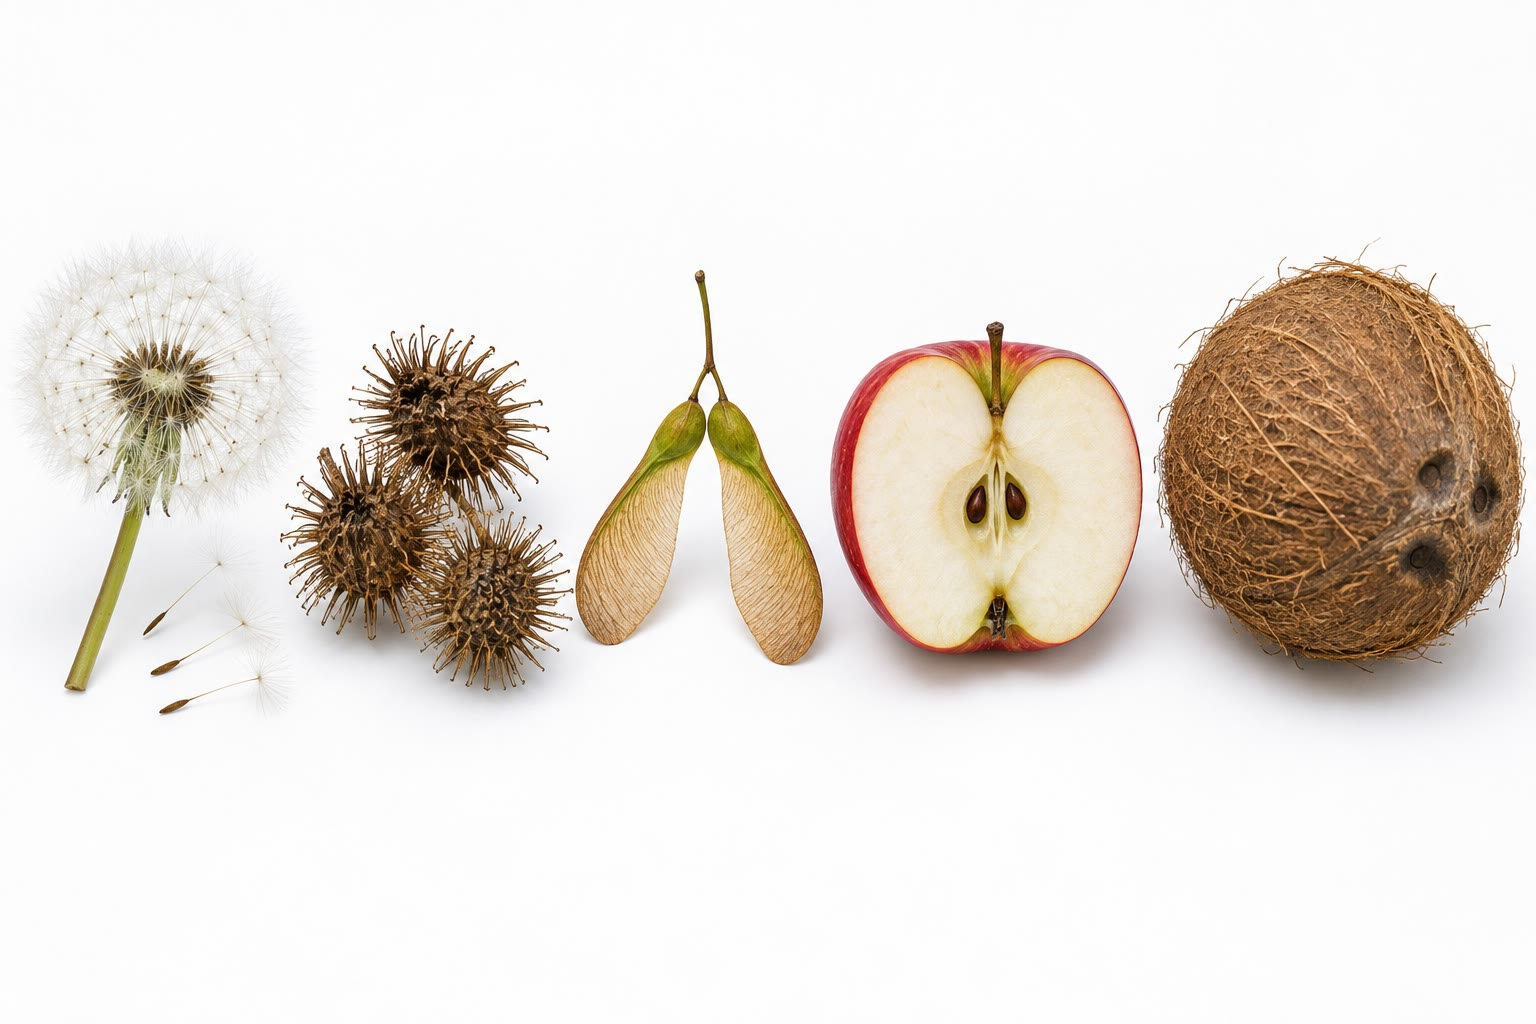
\includegraphics[width=0.62\linewidth]{images/book4/ai/b4-06-fruits-seeds.jpg}

{\small \omterm{def:b2:angiosperm-reproduction:seed}{Buah} yang dibangun untuk penyebaran: payung (rambutan kuning),
kait (arem), sayap (mapel), daging bagi seekor hewan (apel), dan
sabut yang mengapung bagi laut (kelapa).}
\end{omfigure}

\begin{example}[Jarak penyebaran]\label{ex:b2:angiosperm-reproduction:dispersal}
Sebutir akena rambutan kuning dengan payungnya turun pada
\qty{0.3}{m/s}; dari \qty{0.3}{m} di dalam angin \qty{3}{m/s} ia
terbang \qty{3}{m}, dan di dalam arus panas, ratusan meter. Sebuah
samara mapel berputar sendiri turun pada \qty{1}{m/s} dari
\qty{15}{m}: \qty{45}{m}. Sebutir \omterm{def:b2:angiosperm-reproduction:seed}{biji} ceri yang dijatuhkan seekor
burung sesudah terbang dua puluh menit pada \qty{10}{m/s}: sampai
\qty{12}{km}. \omterm{def:b2:angiosperm-reproduction:seed}{Buah} ek jatuh di kakinya sendiri kecuali kalau seekor
jai mengangkutnya, dan jai melakukannya ribuan kali, sejauh satu
kilometer dan lebih, lalu melupakan sepersepuluhnya: pohon ek yang
menjajah kembali Eropa sesudah zaman es terakhir bergerak ke utara
ratusan meter tiap tahun, jauh lebih cepat daripada gelindingan \omterm{def:b2:angiosperm-reproduction:seed}{buah}
ek, dan burunglah yang memindahkannya.
\end{example}

\section{Latihan}

\begin{exercise}[$\star$]\label{exo:b2:angiosperm-reproduction:1}
Sebutkan keempat karangan sebuah \omterm{def:b2:angiosperm-reproduction:flower}{bunga} serta bagian sebuah \omterm{def:b2:angiosperm-reproduction:flower}{benang sari}
dan sebuah \omterm{def:b2:angiosperm-reproduction:flower}{daun buah}. Bagian mana yang \omterm{def:b2:plant-life-cycles:cycles}{sporofit} \omterm{def:b2:meiosis-heredity:meiosis}{diploid}, dan mana yang
\omterm{def:b2:plant-life-cycles:cycles}{gametofit} \omterm{def:b2:meiosis-heredity:meiosis}{haploid}?
\end{exercise}

\begin{exercise}[$\star$]\label{exo:b2:angiosperm-reproduction:2}
Berikan keploidan: sebuah \omterm{def:b2:plant-life-cycles:heterospory}{mikrospora}, sel vegetatifnya, sebuah sel
sperma, sel telurnya, sebuah \omterm{prop:b2:angiosperm-reproduction:embryosac}{inti kutub}, zigotnya, endospermanya, \omterm{def:b2:angiosperm-reproduction:seed}{kulit
bijinya}, dinding \omterm{def:b2:angiosperm-reproduction:seed}{buahnya}.
\end{exercise}

\begin{exercise}[$\star$]\label{exo:b2:angiosperm-reproduction:3}
Daftarkan lima ciri \omterm{def:b2:angiosperm-reproduction:flower}{bunga} yang diserbuki angin dan lima ciri \omterm{def:b2:angiosperm-reproduction:flower}{bunga} yang
diserbuki lebah, lalu berikan sebuah tumbuhan bagi masing-masing.
\end{exercise}

\begin{exercise}[$\star$]\label{exo:b2:angiosperm-reproduction:4}
Apakah \omterm{prop:b2:angiosperm-reproduction:double}{pembuahan ganda} itu, dan apa yang dibuat masing-masing dari
kedua peleburannya? Mengapa endospermanya dapat disebut ``dibuat sesuai
pesanan''?
\end{exercise}

\begin{exercise}[$\star\star$]\label{exo:b2:angiosperm-reproduction:5}
Sehelai rambut jagung panjangnya \qty{25}{cm} dan sebuah \omterm{thm:b2:angiosperm-reproduction:tube}{buluh serbuk
sari} tumbuh pada \qty{1.2}{cm/h}. Berapa lama pembuahannya berlangsung
sesudah \omterm{def:b2:angiosperm-reproduction:pollination}{penyerbukan}? Sebuah malai melepaskan \omterm{def:b2:plant-life-cycles:heterospory}{serbuk sari} dari hari ke-0
sampai hari ke-7 dan rambut tumbuhannya muncul dari hari ke-5 sampai
hari ke-12, seperdelapannya tiap hari; sehelai rambut menangkap \omterm{def:b2:plant-life-cycles:heterospory}{serbuk
sari} hanya selama \omterm{def:b2:plant-life-cycles:heterospory}{serbuk sarinya} dilepaskan. Berapa bagian rambutnya
yang terserbuki?
\end{exercise}

\begin{exercise}[$\star\star$]\label{exo:b2:angiosperm-reproduction:6}
Di bawah \omterm{prop:b2:angiosperm-reproduction:selfing}{ketakserasian sendiri} gametofitik, berapa bagian \omterm{def:b2:plant-life-cycles:heterospory}{serbuk sari}
yang serasi pada persilangan $S_1S_2\times S_1S_2$, $S_1S_2\times
S_1S_3$, $S_1S_2\times S_3S_4$ (putiknya disebut lebih dahulu)?
Berikan \omterm{def:b2:meiosis-heredity:vocabulary}{genotipe} keturunan persilangan yang kedua.
\end{exercise}

\begin{exercise}[$\star\star$]\label{exo:b2:angiosperm-reproduction:7}
Pada sebuah populasi dengan $n$ \omterm{def:b2:meiosis-heredity:vocabulary}{alel} $S$ yang sama frekuensinya, berapa
bagian \omterm{def:b2:plant-life-cycles:heterospory}{serbuk sari} acak yang serasi dengan sebuah tumbuhan tertentu?
Jelaskan mengapa sebuah \omterm{def:b2:meiosis-heredity:vocabulary}{alel} $S$ baru yang muncul lewat \omterm{def:b2:genome-diversification:mutation}{mutasi} menyebar,
dan apa yang diramalkannya bagi cacah \omterm{def:b2:meiosis-heredity:vocabulary}{alelnya}.
\end{exercise}

\begin{exercise}[$\star\star$]\label{exo:b2:angiosperm-reproduction:8}
Sebatang jagung yang \omterm{def:b2:meiosis-heredity:vocabulary}{heterozigot} $Yy$ (endosperma kuning \omterm{def:b2:meiosis-heredity:vocabulary}{dominan})
diserbuki sendiri. Berikan \omterm{def:b2:meiosis-heredity:vocabulary}{genotipe} endosperma bulirnya dan
proporsinya, sambil mengingat bahwa kedua \omterm{prop:b2:angiosperm-reproduction:embryosac}{inti kutubnya} serupa. Berapa
bagian bulirnya yang kuning? Bagaimana kalau tumbuhannya diserbuki
tumbuhan $yy$?
\end{exercise}

\begin{exercise}[$\star\star$]\label{exo:b2:angiosperm-reproduction:9}
Perikanlah percobaan aleuronnya lalu jelaskan apa yang ditunjukkannya
tentang (a) peran lembaganya, (b) peran giberelinnya, (c) tempat
sintesis amilasenya. Mengapa setengah bulir tanpa lembaga adalah
kendali yang penting?
\end{exercise}

\begin{exercise}[$\star\star\star$]\label{exo:b2:angiosperm-reproduction:10}
Bandingkan siasat angin dan hewan dari segi ongkos: tumbuhan yang
diserbuki angin membuat $10^{6}$ butir tiap \omterm{def:b2:plant-life-cycles:heterospory}{bakal biji}, masing-masing
\qty{1}{\micro g}; tumbuhan yang diserbuki hewan membuat $10^{3}$ butir
tiap \omterm{def:b2:plant-life-cycles:heterospory}{bakal biji}, masing-masing \qty{1}{\micro g}, ditambah \qty{5}{mg}
gula \omterm{def:b2:angiosperm-reproduction:pollination}{nektar} tiap \omterm{def:b2:angiosperm-reproduction:flower}{bunga} yang berisi sepuluh \omterm{def:b2:plant-life-cycles:heterospory}{bakal biji}. Hitunglah ongkos
perkembangbiakan tiap \omterm{def:b2:plant-life-cycles:heterospory}{bakal biji} pada tiap kasusnya (ambillah \omterm{def:b2:plant-life-cycles:heterospory}{serbuk
sari} dan gulanya pada energi tiap gram yang sama), lalu jelaskan
mengapa \omterm{def:b2:angiosperm-reproduction:pollination}{penyerbukan} angin tetap bertahan.
\end{exercise}

\begin{exercise}[$\star\star\star$]\label{exo:b2:angiosperm-reproduction:11}
Jelaskan, dengan angka \cref{ex:b2:angiosperm-reproduction:dispersal},
mengapa sebuah \omterm{def:b2:angiosperm-reproduction:seed}{buah} berdaging sepadan dengan ongkosnya bagi sebatang
pohon meskipun hewannya mencerna dagingnya dan menjatuhkan sebagian
besar \omterm{def:b2:angiosperm-reproduction:seed}{bijinya} di tempat yang tidak dapat ditumbuhinya.
\end{exercise}

\begin{exercise}[$\star\star\star$]\label{exo:b2:angiosperm-reproduction:12}
``\omterm{def:b2:angiosperm-reproduction:flower}{Daun buah} yang tertutup adalah alasan tumbuhan berbunga mendominasi
daratan.'' Bahaslah: apa yang dimungkinkan pengurungan \omterm{def:b2:plant-life-cycles:heterospory}{bakal bijinya}
(pemilihan \omterm{def:b2:plant-life-cycles:heterospory}{serbuk sari}, ketakserasian, \omterm{def:b2:angiosperm-reproduction:seed}{buahnya}) dan apa ongkosnya.
\end{exercise}

\section{Soal: Sebuah Kebun dan Sebuah Ladang}

\begin{problem}[{Soal akhir pekan --- penyerbukan sebuah kebun apel
direncanakan berdasarkan ketakserasian sendiri, dan pembuahan serta
hasil sebuah ladang jagung dihitung dari serbuk sari yang dibuatnya,
berakhir pada jadian buah kebunnya dan cacah bulir ladangnya}]
\label{pb:b2:angiosperm-reproduction:1}
Apel bersifat takserasi sendiri secara gametofitik. Sebuah kebun
memiliki tiga varietas: A ($S_1S_2$), B ($S_1S_3$), C ($S_3S_4$).
Sekuntum \omterm{def:b2:angiosperm-reproduction:flower}{bunga} memiliki lima \omterm{def:b2:angiosperm-reproduction:flower}{daun buah} dengan masing-masing dua \omterm{def:b2:plant-life-cycles:heterospory}{bakal
biji}, dan sebuah \omterm{def:b2:angiosperm-reproduction:seed}{buah} yang berbiji kurang dari lima dijatuhkan
pohonnya. Sekali kunjungan lebah menaruh \num{100} \omterm{prop:b2:angiosperm-reproduction:pollen}{butir serbuk sari}
pada sebuah \omterm{def:b2:angiosperm-reproduction:flower}{kepala putik}; tiap butir yang serasi berpeluang $0.1$
membuahi sebuah \omterm{def:b2:plant-life-cycles:heterospory}{bakal biji} yang belum terambil. Sebatang pohon
mengusung \num{5000} \omterm{def:b2:angiosperm-reproduction:flower}{bunga} dan membutuhkan \num{250} \omterm{def:b2:angiosperm-reproduction:seed}{buah} untuk panen
penuh. Jagungnya: sebuah malai melepaskan $10^{7}$ butir selama
\num{7} hari; ladangnya berisi \num{8} tumbuhan tiap meter persegi;
sebatang tumbuhan mengusung satu tongkol berisi \num{600} rambut;
sehelai rambut menyajikan \qty{1e-4}{m^2} kepada \omterm{def:b2:plant-life-cycles:heterospory}{serbuk sari} yang
jatuh; \omterm{def:b2:plant-life-cycles:heterospory}{serbuk sarinya} mengendap pada \qty{0.25}{m/s}; sebutir bulir
memuat \qty{0.3}{g} endosperma.

\medskip
\noindent\textbf{Bagian I --- Keserasiannya.}
\begin{enumerate}
  \item Bagi \omterm{def:b2:plant-life-cycles:heterospory}{serbuk sari} tiap varietasnya pada putik A, berikan bagian
        yang serasi $f$.
  \item Sama untuk putik B dan putik C.
  \item Seekor lebah yang datang dari pohon B menaruh 100 butir pada
        sebuah \omterm{def:b2:angiosperm-reproduction:flower}{kepala putik} A: berapa banyak yang serasi, dan berapa
        \omterm{def:b2:plant-life-cycles:heterospory}{bakal biji} yang diharapkan terbuahi (abaikan penjenuhannya)?
  \item Sama untuk lebah dari C, dan dari sebatang A yang lain.
  \item \omterm{def:b2:angiosperm-reproduction:seed}{Buah} mana yang dipertahankan? Apa risiko menanam sebuah kebun
        varietas A saja?
  \item Sebidang pohon A dikelilingi pohon C; separuh kunjungan
        lebahnya ke A datang dari C. Kalau tiap \omterm{def:b2:angiosperm-reproduction:flower}{bunga} menerima satu
        kunjungan, berapa bagian \omterm{def:b2:angiosperm-reproduction:flower}{bunga} A yang menjadikan \omterm{def:b2:angiosperm-reproduction:seed}{buah}, dan
        berapa \omterm{def:b2:angiosperm-reproduction:seed}{buah} tiap pohonnya? Apakah panennya penuh?
  \item Mengapa kebun menyelang-nyelingkan tanaman apel liar yang
        berbunga berpekan-pekan, dan mengapa \omterm{def:b2:meiosis-heredity:vocabulary}{alel} $S$-nya harus
        diperiksa?
\end{enumerate}

\medskip
\noindent\textbf{Bagian II --- \omterm{def:b2:plant-life-cycles:heterospory}{Serbuk sari} di atas ladang jagungnya.}
\begin{enumerate}[resume]
  \item Hitunglah \omterm{def:b2:plant-life-cycles:heterospory}{serbuk sari} yang dilepaskan tiap meter persegi ladang
        tiap sekon, secara rata-rata sepanjang ketujuh harinya.
  \item Pada keadaan tunak, fluks \omterm{def:b2:plant-life-cycles:heterospory}{serbuk sari} yang mengendap sama
        dengan laju pelepasannya. Hitunglah kepekatan \omterm{def:b2:plant-life-cycles:heterospory}{serbuk sari} di
        udara (butir tiap meter kubik).
  \item Hitunglah cacah butir yang mendarat pada sehelai rambut tiap
        sekon, dan purata waktu tunggu bagi butir pertamanya.
  \item Berapa butir yang diterima sehelai rambut dalam sehari? Mengapa
        hanya yang pertama yang berguna?
  \item Sehelai rambut sepanjang \qty{20}{cm} diserbuki; buluhnya
        tumbuh pada \qty{1}{cm/h}. Kapan \omterm{def:b2:plant-life-cycles:heterospory}{bakal bijinya} dibuahi?
  \item Sebuah kekeringan menunda kemunculan rambutnya lima hari
        sedangkan malainya melepaskan \omterm{def:b2:plant-life-cycles:heterospory}{serbuk sari} sesuai jadwal. Dengan
        memakai masa pelepasan tujuh hari itu, taksirlah bagian musim
        \omterm{def:b2:plant-life-cycles:heterospory}{serbuk sari} yang ditangkap rambutnya, dan akibatnya bagi
        hasilnya.
\end{enumerate}

\medskip
\noindent\textbf{Bagian III --- \omterm{prop:b2:angiosperm-reproduction:double}{Pembuahan ganda} dan bulirnya.}
Ladangnya ditanami varietas berendosperma kuning ($Y$, \omterm{def:b2:meiosis-heredity:vocabulary}{dominan}) di
sebelah ladang putih ($yy$); anginnya bertiup dari ladang putihnya.
\begin{enumerate}[resume]
  \item Berikan \omterm{def:b2:meiosis-heredity:vocabulary}{genotipe} lembaga dan endosperma sebutir bulir sebatang
        tumbuhan $YY$ yang dibuahi \omterm{def:b2:plant-life-cycles:heterospory}{serbuk sari} $yy$.
  \item Apakah bulirnya kuning atau putih? Jelaskan istilah xenia.
  \item Sebatang tumbuhan $Yy$ diserbuki \omterm{def:b2:plant-life-cycles:heterospory}{serbuk sari} $yy$: berikan
        \omterm{def:b2:meiosis-heredity:vocabulary}{genotipe} endospermanya dan frekuensinya.
  \item Endospermanya memuat dua genom dari induknya dan satu dari
        ayahnya. Sebuah gen dengan pengaruh takaran memberi, tiap
        salinannya, 10~satuan pigmen: pigmen apa yang diusung bulir
        $YYy$, $Yyy$, dan $yyY$ (dua takaran dari ayahnya secara
        hipotetis)? Mana di antaranya yang sungguh dapat ada?
  \item Jelaskan mengapa endospermanya, bukan lembaganya, yang kita
        makan, dan berapa bagian massa bulirnya yang diwakilinya kalau
        lembaganya berbobot \qty{0.03}{g}.
  \item Mengapa pembekalan ``sesuai pesanan'' endospermanya merupakan
        keunggulan atas pembekalan gimnosperma?
\end{enumerate}

\medskip
\noindent\textbf{Bagian IV --- Hasilnya.}
\begin{enumerate}[resume]
  \item Kalau \qty{90}{\%} rambutnya terbuahi, hitunglah bulir tiap
        tongkol, tiap tumbuhan, dan tiap meter persegi, serta massa
        endosperma tiap meter persegi.
  \item Ubahlah menjadi ton tiap hektar.
  \item Panenannya memfiksasi \qty{1.2}{kg} karbon tiap meter persegi
        tiap musim, separuhnya berakhir di dalam bulir yang dipanen.
        Periksalah kesepadanannya dengan massa pertanyaan 20
        (endospermanya \qty{45}{\%} karbon).
  \item Berapa \omterm{prop:b2:angiosperm-reproduction:pollen}{butir serbuk sari} yang dilepaskan ladangnya tiap bulir
        yang dipanen?
  \item Jelaskan mengapa sebatang jagung tunggal di sebuah kebun rumah
        menjadikan tongkol yang buruk isinya.
  \item Nyatakan hasilnya: jadian \omterm{def:b2:angiosperm-reproduction:seed}{buah} bidang A dan hasil ladangnya
        dalam bulir tiap meter persegi dan ton tiap hektar.
\end{enumerate}
\end{problem}
